\chapter{Fibre Bundles}\label{chapter:bundles}

    We formulate this chapter in sufficient generality so as to encompass both the topological and smooth setting (or any other one might find useful). To this end we will use the generic terms ''space'', ''group'' and ''morphism''. The reader should choose in which category he wants to work, e.g. topological space, topological group and continuous map in the case of $\mathbf{Top}$.

\section{General bundles}

    \newdef{Bundle}{\index{bundle}\label{diff:bundle}
        A bundle is a triple $(E,B,\pi)$ where $E$ and $B$ are spaces and $\pi$ is a morphism.\footnote{Sometimes one requires that the map $\pi$ is also surjective. However, under this additional restriction we cannot make the association \textbf{Bundle}$(X)\cong\mathbf{C}/X$ of categories anymore.}
    }

    An explicit example in the category $\mathbf{Diff}$ is the following:
    \begin{example}[Fibred manifold]\index{fibred!manifold}\index{fibre}
        A surjective submersion \ref{manifolds:submersion} \[\pi:E\rightarrow B\] where $E$ is called the \textbf{total space}, $B$ the \textbf{base space} and $\pi$ the \textbf{projection}. For every point $p\in B$, the set $\pi^{-1}(p)$ is called the \textbf{fibre over $p$}.
    \end{example}

    The most important example of a bundle is a fibre bundle. Before we can give the definition, we first have to introduce an important tool:
    \newdef{Cocycle}{\index{co-!cycle}\label{diff:G_cocycle}
        Let $B$ be a space and $G$ a group. A ($G$-valued) cocycle on $B$ with values in $G$ with respect to an open cover $\{U_i\}_{i\in I}$ is a family of morphisms $g_{ij}:U_i\cap U_j\rightarrow G$ that satisfy the following condition:
        \begin{gather}
            \label{diff:G_cocycle_condition}
            g_{ij} = g_{ik}\circ g_{kj}.
        \end{gather}
        Two cocycles $(U_i, g_{ij})$ and $(V_i, h_{ij})$ are said to be equivalent if there exist morphisms $\lambda_{i,j}:U_i\cap V_j\rightarrow G$ such that
        \begin{gather}
            \lambda_{i,r}g_{ij}\lambda_{j,s}^{-1} = h_{rs}
        \end{gather}
        whenever this makes sense. The set of cocycles modulo this equivalence relation is denoted by $H^1(B; G)$.\footnote{The notation stems from the fact that this is the first \v{C}ech cohomology group with values in $G$ (see section \ref{section:cech_de_rham}).}
    }
    \begin{property}\label{diff:G_cocycle_conditions}
        Let $\{g_{ij}\}_{i,j\in I}$ be a cocycle on $B$. We have the following properties for all $x\in B$:
        \begin{itemize}
            \item $g_{ij}(x) = (g_{ji}(x))^{-1}$, and
            \item in particular: $g_{ii}(x) = e$.
        \end{itemize}
    \end{property}

    \newdef{Fibre bundle}{\index{fibre!bundle}\index{local!trivialization}\index{structure!group}
        \label{diff:fibre_bundle}
        A fibre bundle is a tuple $(E,B,\pi,F,G)$ where $E,B$ and $F$ are spaces and $G$ is a group (called the \textbf{structure group}), such that there exists a surjective morphism \[\pi:E\rightarrow B\] and an open cover $\{U_i\}_{i\in I}$ of $B$ for which there exists a family of isomorphisms $\{\varphi_i:\pi^{-1}(U_i)\rightarrow U_i\times F\}_{i\in I}$ that make the following diagram commute for all $i\in I$:

        \begin{figure}[ht!]
            \centering
            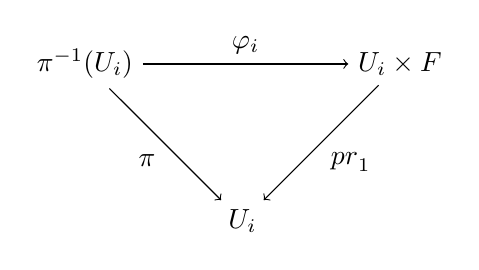
\begin{tikzpicture}
                \node (PI) at (-2, 0) {$\pi^{-1}(U_i)$};
                \node (UF) at (2, 0) {$U_i\times F$};
                \node (U) at (0, -2) {$U_i$};
                \draw[->] (PI) -- node[above]{$\varphi_i$} (UF);
                \draw[->] (PI) -- node[below left]{$\pi$} (U);
                \draw[->] (UF) -- node[below right]{$\text{pr}_1$} (U);
            \end{tikzpicture}
        \end{figure}
        As for general bundles we call $E$ and $B$ the \textbf{total space} and \textbf{base space} respectively. The space $F$ is called the \textbf{(typical) fibre}. We call $(U_i, \varphi_i)$ a \textbf{bundle chart}\footnote{This is due to the similarities with the charts defined for manifolds.} and the set $\{(U_i, \varphi_i)\}_{i\in I}$ a \textbf{local trivialization}\footnote{This name follows from the fact that the bundle is locally isomorphic to a (trivial) product space: $E\cong U\times F$.}. The cover $\{U_i\}_{i\in I}$ itself is called a \textbf{trivializing cover} of the bundle.

        The \textbf{transition maps} $\varphi_j\circ\varphi_i^{-1}:(U_i\cap U_j)\times F\rightarrow (U_i\cap U_j)\times F$ can be identified with the cocycle $g_{ji}:U_i\cap U_j\rightarrow G$, associated to the (left) action (which we require to be faithful\footnote{See definition \ref{group:faithful_action}.}) of $G$ on every fibre, by the following relation:
        \begin{gather}
            \varphi_j\circ\varphi_i^{-1}(b, x) = (b, g_{ji}(b)\cdot x).
        \end{gather}
    }
    \begin{remark}
        One should pay attention that the bundle charts are not coordinate charts in the sense of manifolds \ref{manifolds:chart} because the image of $\varphi_i$ is not an open subset of $\mathbb{R}^n$. However, they serve the same purpose and we can still use them to locally describe the total space $P$.
    \end{remark}
    \begin{notation}
        A fibre bundle $(E,B,\pi,F,G)$ is often denoted by $F\hookrightarrow E\xrightarrow{\ \pi\ }{B}$ or even $\pi:E\rightarrow B$ if the fibre is not important. A drawback of these notations is that we do not immediately know what the structure group of the bundle is.
    \end{notation}

    \newdef{Numerable fibre bundle}{\index{numerable}\label{diff:numerable_bundle}
        A fibre bundle that admits a local trivialization over a numerable open cover.
    }

    \begin{property}[Smooth fibre bundles]
        A smooth fibre bundle is a smooth manifold. This can be proven by combining the local trivializations of the bundle together with the charts of the base and fibre manifolds.
    \end{property}

    \newdef{Compatible\footnotemark\ bundle charts}{\index{compatible!bundle charts}
        \footnotetext{Also called an \textbf{admissible chart}.}
        A bundle chart $(V, \psi)$ is compatible with a trivializing cover $\{(U_i, \varphi_i)\}_{i\in I}$ if whenever $V\cap U_i\neq\emptyset$ there exists a map $h_i:V\cap U_i\rightarrow G$ such that:
        \begin{gather}
            \psi\circ\varphi_i^{-1}(b, x) = (b, h_i(b)x)
        \end{gather}
        for all $b\in V\cap U_i$ and $x\in F$. Two trivializing covers are equivalent if all bundle charts are cross-compatible. As in the case of manifolds, this gives rise to the notion of a \textbf{$G$-atlas}. A \textbf{$G$-bundle} is then defined as a fibre bundle eqipped with an equivalence class of $G$-atlases.
    }

\subsection{Bundle maps}

    \newdef{Bundle map}{\index{bundle!map}
        A bundle map between two fibre bundles $\pi_1:E_1\rightarrow B_1$ and $\pi_2:E_2\rightarrow B_2$ is a pair $(f_E, f_B)$ of morphisms that make diagram \ref{tikz:bundle_map} commute. The map $f_E$ is said to \textbf{cover} $f_B$.

        \begin{figure}[ht!]
        \centering
        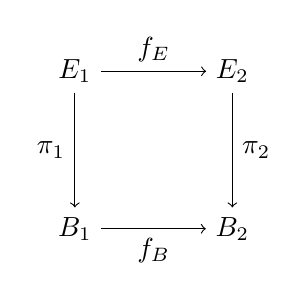
\begin{tikzpicture}
            \node (E1) at (0, 0) {$E_1$};
            \node (E2) at (2, 0) {$E_2$};
            \node (B1) at (0, -2) {$B_1$};
            \node (B2) at (2, -2) {$B_2$};
            \draw[->] (E1) -- node[above]{$f_E$} (E2);
            \draw[->] (E1) -- node[left]{$\pi_1$} (B1);
            \draw[->] (E2) -- node[right]{$\pi_2$} (B2);
            \draw[->] (B1) -- node[below]{$f_B$} (B2);
        \end{tikzpicture}
        \caption{Bundle map between fibre bundles.}
        \label{tikz:bundle_map}
        \end{figure}
    }
    \newdef{Isomorphism}{
        Two fibre bundles $F$ and $G$ are isomorphic if there exist bundle maps $f:F\rightarrow G$ and $g:G\rightarrow F$ such that $f\circ g = \mathbbm{1}_G$ and $g\circ f = \mathbbm{1}_F$.
    }

    \newdef{Equivalent fibre bundles}{\index{gauge!transformation}
        Two fibre bundles $\pi_1:E_1\rightarrow B$ and $\pi_2:E_2\rightarrow B$, with the same typical fibre and structure group, are equivalent if there exist trivializations\footnote{Remark that the collection $\{U_i\}_{i\in I}$ is the same for both trivializations.} $\{(U_i, \varphi_i)\}_{i\in I}$ and $\{(U_i, \varphi'_i)\}_{i\in I}$ such that the associated cocycles are equivalent. An explicit form of the functions $\lambda$ is given by
        \begin{gather}
            \lambda_{i,i} := \varphi_i'\circ\varphi_i^{-1}.
        \end{gather}
    }
    \begin{property}
        Two fibre bundles over the same base space are equivalent if and only if they are isomorphic.
    \end{property}

    \newdef{Trivial bundle}{\index{trivial}\label{manifolds:trivial_bundle}
        A fibre bundle $(E, B, \pi, F)$ is said to be trivial if there exists an equivalence $E \cong B\times F$.
    }

\subsection{Constructions}

    \begin{construct}[Fibre bundle construction theorem]\label{manifolds:theorem:fibre_bundle_construction_theorem}
        Let $M$ and $F$ be topological spaces and let $G$ be a topological group equipped with a left action on $F$. Suppose that we are given a cover $\{U_i\}_{i\in I}$ of $M$ and a set of continuous functions $\{g_{ji}:U_i\cap U_j\rightarrow G\}$ that satisfy the cocycle condition \ref{diff:G_cocycle}. A fibre bundle over $M$ can then be constructed as follows:
        \begin{enumerate}
            \item We first construct for every set $U_i$ an associated set $U_i\times F$.
            \item We then construct the disjoint union $T:=\bigsqcup_{i\in I}U_i\times F$ and equip it with the disjoint union topology (see definition \ref{topology:disjoint_union}).
            \item From this disjoint union we construct a quotient space and equip it with the quotient space topology (see definition \ref{topology:quotient_space}). For this we define the following equivalence relation for every $i, j\in I$:
                \begin{gather}
                    (p, f)\sim(p, g_{ji}(x)\cdot f)
                \end{gather}
                for all $x\in U_i\cap U_j$ and $f\in F$.
            \item The fibre bundle is equal to the quotient space $T/\sim$ together with the projection $\pi$ that maps the equivalence class of $(x, f)\in T$ to $x\in M$.
            \item Local trivializations are given by the maps $\varphi_i:\pi^{-1}(U_i)\rightarrow U_i\times F$ that satisfy
                \begin{gather}
                    \varphi_i^{-1}:(x, f)\mapsto [(x, f)]
                \end{gather}
                where $[A]$ denotes the equivalence class of $A$ in $T/\sim$.
        \end{enumerate}
    \end{construct}
    \begin{property}[Homotopy invariance]
        Homotopic transition functions give rise to equivalent (and hence isomorphic) bundles. (This follows from the homotopy invariance of \v{C}ech cohomology.)
    \end{property}

    \begin{remark}[Clutching]\index{clutching}
        The above construction is often called the clutching construction, especially when constructing vector bundles over a sphere $S^n$. There the covering consists of two hemispheres that intersect on the equator $S^{n-1}$ and the function $g_{21}$ is then also called the \textbf{clutching function}.
    \end{remark}
    \begin{property}[Vector bundles over a sphere]\index{vector!bundle}\label{diff:vector_bundles_over_sphere}
        The clutching theorem and the homotopy invariance imply that vector bundles over the sphere are determined by homotopy classes of functions $S^{n-1}\rightarrow\text{GL}_p(k)$, i.e. they are classified by the homotopy group $\pi_{n-1}(\text{GL}_p(k))$.
    \end{property}

    \newdef{Subbundle}{\index{sub!bundle}
        A subbundle of a fibre bundle $\pi:E\rightarrow B$ is a triple $(E',B',\pi')$ such that $E'\subset E$, $B'\subset B$ and $\pi' = \pi|_{E'}$ (where $\subset$ denotes an inclusion morphism in the surrounding category).
    }
    \newdef{Pullback bundle}{\index{pullback!bundle}\label{manifolds:pullback_bundle}
        Let $\pi:E\rightarrow B$ be a fibre bundle and let $f:B'\rightarrow B$ be a morphism of spaces. The pullback bundle $f^*E$ is defined as follows:
        \begin{gather}
            f^*E := \big\{(b', e)\in B'\times E:f(b') = \pi(e)\big\}.
        \end{gather}
        The topology on $f^*E$ is induced by the subspace topology of the product $B'\times E$. The projection onto the second factor gives a map of total spaces $f^*E\rightarrow E$.
    }

    \newdef{Fibre product}{\index{fibre!product}
        Let $(F_1,B,\pi_1)$ and $(F_2,B,\pi_2)$  be two fibre bundles on a base space $B$. Their fibre product is defined as follows:
        \begin{gather}
            \label{manifolds:fibre_product}
            F_1\diamond F_2 := \big\{(f, g)\in F_1\times F_2: \pi_1(f) = \pi_2(g)\big\}.
        \end{gather}
    }

\subsection{Sections}

    \newdef{Section}{\index{section}
        A (\textbf{global}) section of a fibre bundle $\pi:E\rightarrow B$ is a morphism $s:B\rightarrow E$ such that $\pi\circ s = \mathbbm{1}_B$. For any open subset $U\subset B$ we define a \textbf{local} section as a morphism $s_U:U\rightarrow E$ such that $\pi\circ s_U(b) = b$ for all $b\in U$.
    }
    \begin{notation}
        \nomenclature[O_Gamma]{$\Gamma(E)$}{set of global sections of a fibre bundle $E$}
        The set of all global sections of a bundle $E$ is denoted by $\Gamma(E)$. The set of local sections over $U$ is sometimes denoted by $\Gamma(U, E)$. With this latter notation we see that $\Gamma(E)\equiv\Gamma(B, E)$.
    \end{notation}

    \begin{property}
        The sections of a fibre bundle $E$ pullback to the pullback bundle $f^*E$ by setting $f^*s := s\circ f$.
    \end{property}

\section{Vector bundles}
	The tangent space and tangent bundle, as introduced in subsection \ref{diff:section:tangent_space}, can also be introduced in a more topological way:
	
\subsection{Tangent bundles}

	\begin{construct}[Tangent bundle]\index{tangent!bundle}
		Let $M$ be a manifold with atlas $\{(U_i, \varphi_i)\}_{i\leq n}$. Consider for every open set $U$ an associated set $TU = U\times\mathbb{R}^n$. For every smooth function $f$ we can define an associated smooth function on $TU$, called the differential of $f$, by:
		\begin{equation}
			\label{diff:manifolds:T_function}
			Tf:U\times\mathbb{R}^n\rightarrow f(U)\times\mathbb{R}^n:(x, v)\mapsto(f(x), Df(x)v)
		\end{equation}
		where $Df(x):\mathbb{R}^n\rightarrow\mathbb{R}^n$ is the linear operator associated with the Jacobian matrix of $f$ in $x$. Applying this definition to the transition functions $\psi_{ji}$ we obtain a new set of functions $\widetilde{\psi}_{ji} := T\psi_{ji}$ given by:
		\begin{equation}
			\widetilde{\psi}_{ji}(\varphi_i(x), v) = \left(\varphi_j(x), (\varphi_j\circ\varphi_i^{-1})'(\varphi_i(x))v\right)
		\end{equation}
		Because the transition functions are diffeomorphisms the Jacobians are invertible. This implies that the maps $\widetilde\psi_{ji}$ are elements of $GL(\mathbb{R}^n)$. The tangent bundle is now obtained by applying the fibre bundle construction theorem \ref{manifolds:theorem:fibre_bundle_construction_theorem} to the triple $(M, \mathbb{R}^n, GL(\mathbb{R}^n))$ together with the cover $\{U_i\}_{i\leq n}$ and the cocycle $\{\widetilde\psi_{ji}\}_{i,j\in I}$.
	\end{construct}
	\begin{remark*}
		The charts in the atlas of the constructed bundle are sometimes called \textbf{natural charts}.
	\end{remark*}
	
	\begin{property}
		Let $M$ be an $n$-dimensional manifold. Using the natural charts on $TM$ which give a local homeomorphism \[\psi_i:TM\rightarrow U_i\times\mathbb{R}^n\cong\mathbb{R}^n\times\mathbb{R}^n\] we can see that $TM$ is isomorphic to $\mathbb{R}^{2n}$. This implies that the tangent bundle is a manifold of dimension $2n$.
	\end{property}
	
	\newdef{Tangent space}{\index{tangent!space}
		Let $x\in M$. The topological definition of the tangent space is given by the fibre
		\begin{equation}
			T_xM := \tau_M^{-1}(x)
		\end{equation}
		If we use the natural charts to map $T_xM$ to the set $\varphi_i(x)\times\mathbb{R}^n$, we see that $T_xM$ is isomorphic to $\mathbb{R}^n$ and thus also to $M$ itself. Furthermore, we can equip every fibre with the following vector space structure:
		\begin{align*}
			(x, v_1)+(x, v_2)&:=(x, v_1 + v_2)\\
			r(x, v)&:=(x, rv)
		\end{align*}
	}
	\begin{remark}
		Now it is clear that the rule "\textit{a vector is something that transforms like a vector}" stems from the fact that:
		\[\text{a vector }v\in T_xM\text{ is tangent to }\varphi_i(x)\text{ in a chart }(U_i, \varphi_i)\]
		if and only if
		\[D(\varphi_j\circ\varphi_i^{-1})(\varphi_i(x))v\text{ is tangent to }\varphi_j(x)\text{ in a chart }(U_j, \varphi_j)\]
		Comparing this property to \ref{diff:manifolds:tangent_curve_transformation}, we see that tangent vectors defined through equivalence classes of tangent curves are indeed tangent vectors according to our new construction.
	\end{remark}
	
	\newdef{Differential}{\index{differential}\label{manifolds:differential}
		The map $T$ from \ref{diff:manifolds:T_function} can be generalized to arbitrary smooth manifolds as the map $Tf:TM\rightarrow TN$. Furthermore, let $x\in U\subseteq M$ and let $V = f(U)$. By looking at the restriction of $Tf$ to $T_xM$, denoted by $T_xf$, we see that it maps $T_xU$ to $T_{f(x)}V$ (where $V=f(U)$) linearly. So $T_xf$ is a linear map on fibres.
	}
	
	\begin{property}
		The map $Tf: TM\rightarrow TN$ (see \ref{diff:manifolds:T_function}) has following properties\footnotemark:
		\begin{itemize}
			\item $T(\mathbbm{1}_M) = \mathbbm{1}_{TM}$
			\item Let $f, g$ be two smooth functions on smooth manifolds. Then $T(f\circ g) = Tf\circ Tg$.
		\end{itemize}
	\end{property}
	\footnotetext{This turns the map $T$ into a functor on the category of smooth manifolds. We can view $T$ as a functorial derivative.}
	
	\begin{remark*}
		We can also use a construction similar to that of the tangent bundle to reconstruct the original manifold $M$ from the sets $\varphi_i(U_i)$.
	\end{remark*}
	
	\newdef{Rank}{\index{rank}
		\label{manifolds:rank}
		Let $f:M\rightarrow N$ be a differentiable map between smooth manifolds. Using the fact that $Tf$ is a linear map of fibres\footnotemark, we define the rank of $f$ at $p\in M$ as the rank (as in \ref{linalgebra:image_rank}) of the differential $Tf:T_pM\rightarrow T_{f(p)}N$.
	}
	\footnotetext{See definition \ref{manifolds:differential}.}
	
	\begin{theorem}[Inverse function theorem]\index{inverse function theorem}\label{manifolds:theorem:inverse_function_theorem}
		A $C^\infty$ map $f:M\rightarrow N$ between smooth manifolds is locally homeomorphic (resp. locally diffeomorphic) if and only if its differential $Tf:T_pM\rightarrow T_pN$ is an isomorphism (resp. diffeomorphism) at $p$.
	\end{theorem}

\subsection{Vector bundles}

	Instead of restricting ourselves by letting the typical fibre be a Euclidean space with the same dimension as the base manifold, we can generalize the construction of the tangent bundle in the following way:
		
	\begin{construct}[Vector bundle]\index{vector!bundle}\index{fibre}\index{local!trivialization}
		\label{manifolds:vector_bundle_construction}
		Consider a smooth $n$-dimensional manifold $M$ with atlas $\{(U_i, \varphi_i)\}_{i\leq n}$, a cocycle $\{g_{ji}: U_i\cap U_j\rightarrow G\}_{i,j\leq n}$ with values in a Lie group $G$ and a smooth representation $\rho:G\rightarrow GL(V)$, where $V$ is a vector space.
		
		Now we can construct a new topological space $E$, similar to the construction of the tangent bundle, by taking the disjoint union of the sets $\varphi_i(U_i)\times V$ and quotienting out using the functions $\widetilde{g}_{ji}:(\varphi_i(x), v)\mapsto(\varphi_j(x), g_{ji}(x)\cdot v)$, where $g\cdot v\equiv \rho(g)v$. This gives us a set of natural charts\footnotemark\ $\{(\widetilde{U}_i, \widetilde{\varphi}_i)\}_{i\leq n}$, a projection map $\pi:E\rightarrow M$ induced by the local projection $\varphi_i(U_i)\times V\rightarrow\varphi_i(U_i)$ and a naturally defined vector space on every fibre $V_x:=\pi^{-1}(x)$. Furthermore every fibre $V_x$ is (although not necessarilly canonically) isomorphic to $V$.
		
		This set $E$ is called a \textbf{smooth vector bundle} over $M$ with \textit{typical fibre} $V$ and \textit{projection map} $\pi$.
		\footnotetext{We could instead use any other kind of topological space. The point is that a vector bundle is a fibre bundle \ref{manifolds:fibre_bundle} for which the typical fibres are vector spaces.}
	\end{construct}

	\begin{remark}
		As is also the case for tangent bundles (which are specific cases of vector bundles where the typical fibre has the same dimension as the manifold) the choice of charts on $E$ is not random. To preserve the structure of fibres, the use of the natural charts is imperative.
	\end{remark}
	\begin{remark}
		Vector bundles are smooth fibre bundles where the typical fibre is a vector space $V$ and the structure group is given by $GL(V)$.
	\end{remark}
	
	\newdef{Associated vector bundle}{\label{manifolds:associated_vector_bundle}
		Consider a representation\newline $\rho:GL(\mathbb{R}^n)\rightarrow GL(\mathbb{R}^l)$ and the cocycle $t_{ji} := D(\psi_{ji})\circ\varphi_i$ as defined for tangent bundles. The composition $\rho\circ t_{ji}:U_i\cap U_j\overset{t_{ji}}{\rightarrow} GL(\mathbb{R}^n) \overset{\rho}{\rightarrow} GL(\mathbb{R}^l)$ is again a cocycle and can thus be used to define a new vector bundle on $M$. The vector bundle $E = \rho(TM)$ so obtained is called the associated bundle of the tangent bundle induced by $\rho$.
	}
	\begin{remark}
		\label{manifolds:vector_principal_correspondence}
		It should also be noted that every vector bundle is associated to a principle $GL(V)$-bundle where the cocycles $g_{ji}$ now act by left multiplication on elements of $GL(V)$.
	\end{remark}

	\begin{example}[Contravariant vectors]\index{contravariant}
		By noting that the $k^{th}$ tensor power $\otimes^k$ induces a representation given by the tensor product of the representations, we can construct the bundle of $k^{th}$ order contravariant vectors $\otimes^k(TM)$ with the cocycle given by $x\mapsto t_{ji}(x)\otimes\cdots\otimes t_{ji}(x)$.
	\end{example}
	\begin{example}[Cotangent bundle]\index{covariant}\label{manifolds:cotangent_bundle}
		Another (smooth) representation is given by $A\mapsto (A^T)^{-1}=(A^{-1})^T$ for every linear map $A$. The vector bundle constructed this way, where the cocycle is given by $(t_{ji}^T)^{-1}$, is called the cotangent bundle on $M$ and is denoted by $T^*M$. Elements of the fibres are called covariant vectors or covectors.
	\end{example}
	\begin{notation}
		A combination of the cocycle $t_{ji}$ and its dual $(t_{ji}^T)^{-1}$ can also be used to define the bundle of $k^{th}$ order contravariant and $l^{th}$ order covariant vectors on $M$. This bundle is denoted by $T^{(k, l)}M$.
	\end{notation}
	
	\begin{example}[Pseudovectors]\index{pseudovector}
		If we consider the representation
		\begin{equation}
			\rho:A\mapsto \sgn\det(A)A
		\end{equation}
		we can construct a bundle similar to the tangent bundle. The sign of the cocycle functions $t_{ji}$ now has an influence on the fibres. Elements of these fibres are called \textbf{pseudovectors}.
	\end{example}
	
	\newdef{Subbundle}{\index{subbundle}
		A subbundle of a vector bundle $\pi:E\rightarrow M$ is a collection of subspaces $U_x$ of fibres $E_x$ that make up a vector bundle on their own.
	}
	
	\newdef{Whitney sum}{\index{Whitney!sum}
		Consider two vector bundles $W, W'$ with fibres $E, E'$ respectively. Then we can construct a new vector bundle $W\oplus W'$ by defining the new typical fibre to be the direct sum $E\oplus E'$, i.e. the fibre above b is given by $E_b\oplus E_b'$.  This operation is called the Whitney sum or direct sum of vector bundles.
	}
	
\subsection{Sections}
	\begin{remark*}
		Vector fields can be regarded as sections of the tangent bundle. Similarly, 1-forms can be regarded as sections of the cotangent bundle.
	\end{remark*}
	
	\newdef{Frame}{\index{frame}\label{diff:frame}
		A frame of a vector bundle $E$ is a tuple $(s_1, ..., s_n)$ of smooth sections such that $(s_1(b), ..., s_n(b))$ is a basis of the fibre $\pi^{-1}(b)$ for all $b\in B$.
	}
	\begin{property}
		A vector bundle is trivial if and only if there exists a frame of global sections.
	\end{property}

\section{Vector fields}
	\newdef{Vector field}{\index{vector!field}
		A smooth section $s\in\Gamma(TM)$ of the tangent bundle is called a vector field.
	}
	\begin{notation}
		The set of all vector fields on a manifold $M$ is often denoted by $\mathfrak{X}(M)$.
	\end{notation}
	
	\newdef{Pullback}{\index{pullback}
		Let $X$ be vector field on $M$ and let $\varphi:M\rightarrow N$ be a diffeomorphism between smooth manifolds. The pullback of $X$ along $\varphi$ is defined as:
		\begin{equation}
			\label{manifolds:pullback}
			(\varphi^*X)_p = T\varphi^{-1}(X_{\varphi(p)})
		\end{equation}
	}
	\newdef{Pushforward}{\index{pushforward}
		Let $X\in\mathfrak{X}(M)$ and let $\varphi:M\rightarrow N$ be a diffeomorphism between smooth manifolds. Using the differential $T\varphi$ we can define the pushforward of $X$ along $\varphi$ as:
		\begin{equation}
			\label{manifolds:pushforward}
			(\varphi_*X)_{\varphi(p)} = T\varphi(X_p)
		\end{equation}
		which we can rewrite using the pullback as:
		\begin{equation}
			\label{manifolds:pullback_pushforward}
			\varphi_*X = \varphi^{-1*}X
		\end{equation}
		Or equivalently we can define a vector field on $N$ by:
		\begin{equation}
			(\varphi_*X)_q(f) = X_{\varphi^{-1}(q)}(f\circ\varphi)
		\end{equation}
		for all smooth functions $f:N\rightarrow\mathbb{R}$ and points $q\in N$.
	}
	
	\begin{remark*}
		For both the pullback and pushforward, we need the map $\varphi$ to be a diffeomorphism. For differential forms this is only necessary for the definition of pushforwards. (See definitions \ref{forms:pullback} and \ref{forms:pushforward}).
	\end{remark*}
	
\subsection{Integral curves}
	\newdef{Integral curve}{\index{integral!curve}
		Let $X\in\mathfrak{X}(M)$ and let $\gamma:\ ]a, b[\rightarrow M$ be a smooth curve on $M$. $\gamma$ is said to be an integral curve of $X$ if:
		\begin{equation}
			\label{manifolds:integral_curve}
			\boxed{\gamma'(t) = X(\gamma(t))}
		\end{equation}
		for all $t\in]a,b[$ where we defined $\gamma'(t) := T\gamma(t, 1)$ using the functorial derivative \ref{diff:manifolds:T_function}.
		
		This equation can be seen as a system of ordinary differential equations in the second argument. Using Picard's existence theorem\footnotemark\ together with the initial value condition $\gamma(0) = p$ we can find a unique curve on $]a, b[$ satisfying the defining equation \ref{manifolds:integral_curve}. Furthermore we can extend the interval $]a, b[$ to a maximal interval such that the solution is still unique. This solution, denoted by $\gamma_p$, is called the \textbf{integral curve of $X$ through $p$}.
		\footnotetext{Also Picard-Lindel\"of theorem.}
	}
	
	\newdef{Flow}{\index{flow}
		Let $X\in\mathfrak{X}(M)$. The function $\sigma_t$:
		\begin{equation}
			\label{manifolds:flow}
			\sigma_t(p) = \gamma_p(t)
		\end{equation}
		is called the flow of $X$ at time $t$. The flow domain is defined as the set $D(X) = \{(t, p)\in\mathbb{R}\times M\ |\ t\in ]a_p, b_p[\}$ where $]a_p, b_p[$ is the maximal interval on which $\gamma_p(t)$ is defined.
	}
	\begin{property}
		Suppose that $D(X) = \mathbb{R}\times M$. The flow $\sigma_t$ has following properties for all $s, t\in\mathbb{R}$:
		\begin{itemize}
			\item $\sigma_0 = \mathbbm{1}_M$
			\item $\sigma_{s+t} = \sigma_s\circ\sigma_t$
			\item $\sigma_{-t} = (\sigma_t)^{-1}$
		\end{itemize}
		These three properties\footnote{The third property follows from the other two.}\ say that $\sigma_t$ is a bijective group action from $M$ to the additive group of real numbers. This implies that $\sigma_t$ is indeed a \textbf{flow} in the general mathematical sense.
	\end{property}
	
	\newdef{Complete vector field}{\index{complete!vector field}
		A vector field $X$ is called complete if the flow domain for every flow is whole $\mathbb{R}$.
	}
	
	\begin{property}
		The flow $\sigma_t$ of a vector field is of class $C^\infty$. If $X$ is complete it follows from previous definition that the flow is a diffeomorphism from $M$ onto itself.
	\end{property}

	
\subsection{Lie derivative}

	\newformula{Lie derivative for smooth functions}{\index{Lie!derivative}
		Let $X\in\mathfrak{X}(M)$ and let $f:M\rightarrow\mathbb{R}$ be a smooth function. The Lie derivative of $f$ with respect to $X$ at $p\in M$ is defined as:
		\begin{equation}
			\label{manifolds:lie_derivative_functions}
			\boxed{(\mathcal{L}_Xf)(p) = \lim_{t\rightarrow0}\stylefrac{f(\gamma_p(t)) - f(p)}{t}}
		\end{equation}
		which closely resembles the standard derivative in Euclidean space.
	}
	
	\begin{formula}[$\dag$]\label{manifolds:ex:lie_derivative_function}
		Working out previous formula and rewriting it as an operator equality gives:
		\begin{equation}
			\label{manifolds:lie_derivative_function_expansion}
			\boxed{\mathcal{L}_X = \sum_kX_k\pderiv{}{x^k}}
		\end{equation}
		It is clear that this is just the vector field $X$ expanded in the basis \ref{diff:manifolds:tangent_vector_partial}. We also recover the behaviour of a tangent vector as a derivation. So for smooth functions $f:M\rightarrow\mathbb{R}$ we obtain:
		\begin{equation}
			\mathcal{L}_Xf(p) = X_p(f)
		\end{equation}
	\end{formula}
	
	\newformula{Lie derivative for vector fields$^\dag$}{\label{manifolds:ex:lie_derivative_vector_fields}
		Let $X, Y\in\mathfrak{X}(M)$
		\begin{equation}
			\label{manifolds:lie_derivative_vector_field}
			\boxed{\mathcal{L}_XY = \left.\deriv{}{t}(\sigma_t^*X)(\gamma_p(t))\right|_{t=0}}
		\end{equation}
	}
	\begin{property}\index{Lie!bracket}
		Let $X, Y\in\mathfrak{X}(M)$ be vector fields of class $C^k$. The Lie derivative has following properties:
		\begin{itemize}
			\item $\mathcal{L}_XY$ is a vector field.
			\item \textbf{Lie bracket}:
				\begin{equation}
					\label{manifolds:lie_bracket}
					\mathcal{L}_XY = [X, Y]
				\end{equation}
				which is also a derivation on $C^{k-1}(M, \mathbb{R})$ due to the cancellation of second-order derivatives in the local representation.
			\item The Lie derivative is antisymmetric:
				\begin{equation}
					\mathcal{L}_XY = -\mathcal{L}_YX
				\end{equation}
				This follows from the previous property.
		\end{itemize}
	\end{property}
	
\subsection{Frobenius theorem}

	Looking at property \ref{linalgebra:grassmannian_construction} and noting that GL$_n(\mathbb{C})$ is a Lie group, we can endow the Grassmannian Gr$(k, \mathbb{R}^n)$ \ref{linalgebra:grassmannian} with a differentiable structure, turning it into a smooth manifold. With this we can construct a new bundle\footnotemark\ by applying the usual 'gluing' process:
	\footnotetext{Due to the fact that the Grassmannian is not a vector space, we construct a general fibre bundle and not a vector bundle.}
	
	\begin{construct}[Grassman bundle]\index{Grassman!bundle}
		First define the transition functions:
		\begin{equation}
			\psi_{ji}:\varphi_i(U_i\cap U_j)\times \text{Gr}(k, \mathbb{R}^n) \rightarrow \varphi_j(U_i\cap U_j)\times \text{Gr}(k, \mathbb{R}^n):(\varphi_i(x), V)\mapsto(\varphi_j(x), t_{ji}(x)\cdot V)
		\end{equation}
		where $\{t_{ji}\}_{i, j\leq n}$ is the tangent bundle cocycle, but now with an action on the compact manifold Gr$(k, \mathbb{R}^n)$ instead of the vector space $\mathbb{R}^n$. Using this set of transition functions we use a construction similar to \ref{manifolds:vector_bundle_construction} to create a new (fibre) bundle where every fibre is diffeomorphic to Gr$(k, \mathbb{R}^n)$, namely it is the Grassmannian Gr$(k, T_pM)$ associated to the tangent space in every point $p\in M$.
	\end{construct}
	\begin{notation}
		The Grassman $k$-plane bundle is denoted by Gr$(k, TM)$.
	\end{notation}
	
	\newdef{Distribution}{\index{distribution!of $k$-planes}\label{manifolds:distribution}
		A smooth section of the Grassman $k$-plane bundle is called a distribution of $k$-planes.
	}
	
	\begin{definition}[Integrable]\index{integrable!manifold}
		Let $M$ be a smooth manifold and let $W\in\Gamma(\text{Gr}(k, TM))$ be a distribution of $k$-planes. A submanifold $N\subseteq M$ is said to integrate $W$ with initial condition $p_0\in M$ if for every $p\in N$ we find that $W(p) = T_pN$ and $p_0\in N$. $W$ is said to be integrable if there exists such a submanifold $N$.
	\end{definition}
	
	\newdef{Frobenius integrability condition}{\index{Frobenius!integrability condition}
		A distribution of $k$-planes $W$ over a smooth manifold $M$ is said to satisfy the Frobenius integrability condition in an open set $U\subseteq M$ if for every two vector fields $X, Y$ defined on $U$, such that $X(p)\in W(p)$ and $Y(p)\in W(p)$ for all $p\in U$, there Lie bracket $[X, Y](p)$ is also an element of $W(p)$ for all $p\in U$.
	}
	\begin{theorem}[Frobenius' integrability theorem]\index{Frobenius!integrability theorem}\label{manifolds:frobenius}
		Let $W$ be a distribution of $k$-planes over a smooth manifold $M$. Then $W$ is integrable if and only if $W$ satisfies the Frobenius integrability condition.
	\end{theorem}

\section{Differential \texorpdfstring{$k$}{k}\ -forms}

	\newdef{Differential form}{\index{differential form}
		A differential $k$-form is a map
		\begin{equation}
			\boxed{\omega: T^{\diamond k}M\rightarrow \mathbb{R}}
		\end{equation}
		such that the restriction of $\omega$ to each fibre of the fibre product\footnotemark\ $T^{\diamond k}M$ is multilinear and antisymmetric.
		
		The space of all differential $k$-forms on a manifold $M$ is denoted by $\Omega^k(M)$. $\Omega^0(M)$ is defined as the space of smooth functions $C^\infty:M\rightarrow\mathbb{R}$.
	}
	\footnotetext{See definition \ref{manifolds:fibre_product}.}
	
	\begin{adefinition}
		An alternative definition goes as follows. Consider the representation \[\rho_k:GL(R^{m*})\rightarrow GL(\Lambda^k(\mathbb{R}^{m*})): T\mapsto T\wedge...\wedge T\] where $T$ is a linear map. This representation induces an associated vector bundle\footnotemark\ $\rho_k(\tau_M^*)$ of the cotangent bundle on $M$. A differential $k$-form is then given by a section of $\rho_k(\tau_M^*)$. $\Omega^k(M)$ can then be defined as follows: \[\Omega^k(M) = \Gamma(\rho_k(\tau_M^*))\]
	\end{adefinition}
	\footnotetext{See definition \ref{manifolds:associated_vector_bundle}.}
	
	\begin{construct}
		We can construct a graded algebra by equipping the graded vector space
		\begin{equation}
			\Omega(M) = \bigoplus_{k\geq0}\Omega^k(M)
		\end{equation}
		with the wedge product of differential forms (which is induced by the wedge product on $\Lambda^k(\mathbb{R}^{m*})$ through the alternative definition). This graded algebra is associative, graded-commutative and unital with the constant function $1\in C^{\infty}(M)$ as identity element.
	\end{construct}

	\newdef{Pullback}{\index{pullback}
		Let $f:M\rightarrow N$ be a smooth function between smooth manifolds and let $\omega$ be a differential $k$-form on $N$. The pullback of $\omega$ by $f$ is defined as:
		\begin{equation}
			\label{forms:pullback}
			\boxed{f^*(\omega) = \omega\circ Tf:TM\rightarrow\mathbb{R}}
		\end{equation}
		So $f^*$ can be seen as a map pulling elements from $T^*N$ back to $T^*M$.
	}
	\newdef{Pushforward}{\index{pushforward}
		Let $f:M\rightarrow N$ be a diffeomorphism between smooth manifolds and let $\omega$ be a differential $k$-form on $M$. The pushforward $\omega$ by $f$ is defined as:
		\begin{equation}
			\label{forms:pushforward}
			f_*(\omega): \omega\circ Tf^{-1}: TN\rightarrow\mathbb{R}
		\end{equation}
		or using the pullback:
		\begin{equation}
			f_*(\omega) = f^{-1*}(\omega)
		\end{equation}
	}
	\begin{remark*}
		Note that the pushforward of differential $k$-form is only defined for diffeomorphisms, in constrast to pullbacks which only require smooth functions. Furthermore this also explains why differential forms are the most valuable elements in differential geomeotry. Vector fields can't even be pulled back in general by smooth maps.
	\end{remark*}
	
	\newformula{Dual basis}{\index{basis}
		Consider the basis $\{\left.\pderiv{}{x_i}\right|_p\}_{i\leq n}$ from definition \ref{diff:manifolds:tangent_vector_partial} for the tangent space $T_pM$. From this set we can construct a natural dual basis for the cotangent space $T_p^*M$ using the natural pairing of these spaces:
		\begin{equation}
			\label{forms:basis}
			\left\langle\pderiv{}{x_i}, dx_j\right\rangle = \delta_{ij}
		\end{equation}
	}
	
\subsection{Exterior derivative}

	\newdef{Exterior derivative}{\index{exterior!derivative}\index{differential}\label{forms:def:exterior_derivative}
		The exterior derivative $d_k$ is a map defined on the graded algebra of differential $k$-forms:
		\begin{equation}
			d_k:\Omega^k(M)\rightarrow\Omega^{k+1}(M)
		\end{equation}
		For $k=0$ it is given by\footnotemark:
		\begin{equation}
			\label{forms:function_derivative}
			df = \sum_{i=1}^n\pderiv{f}{x_i}dx_i
		\end{equation}
		where we remark that the `infinitesimals' are in fact unit vectors with norm $1$. This formula can be generalized to higher dimensions as follows:
		\begin{equation}
			\label{forms:exterior_derivative}
			\boxed{d(fdx_{i_1}\wedge...\wedge dx_{i_k}) = df\wedge dx_{i_1}\wedge...\wedge dx_{i_k}}
		\end{equation}
	}
	\footnotetext{For $f\in\Omega^0(M)$, we call $df$ the \textbf{differential} of $f$.}
	
	\begin{result}
		It follows immediately from \ref{forms:exterior_derivative} that
		\begin{equation}
			d(dx_i) = 0
		\end{equation}
		for all $i\leq n$.
	\end{result}
	
	\begin{property}\index{Leibniz!rule}\label{forms:exterior_derivative_properties}
		The exterior derivatives have following properties:
		\begin{itemize}
			\item For all $k\geq 0$, for all $\omega\in\Omega^k(M)$: $d_k\circ d_{k+1} = 0$, so $\text{im}(d_k)\subseteq\text{ker}(d_{k+1})$.
			\item The exterior derivative is an $\mathbb{R}$-linear map.
			\item Graded Leibniz rule:
				\begin{equation}
					d(\omega_1\wedge\omega_2) = d\omega_1\wedge\omega_2 + (-1)^j\omega_1\wedge d\omega_2
				\end{equation}
				where $\omega_1\in\Omega^j(M), \omega_2\in\Omega^k(M)$.
			\item Let $f\in C^\infty(M)$: $f^*(d\omega) = d(f^*\omega)$ where $f^*$ denotes the pullback \ref{forms:pullback}.
		\end{itemize}
	\end{property}
	
	\begin{remark}[$\dag$]\index{gradient}\index{rotor}\index{divergence}\label{forms:vector_calculus}
		The gradient, rotor (curl) and divergence from standard vector calculus\footnote{See section \ref{vectorcalculus:nabla}.} can be rewritten using exterior derivatives as follows: Let $\vector{f} = (f_1, f_2, f_3)$ with $f_i$ smooth for every $i$ and let $f$ be a smooth function. Denote the canonical isomorphism between $\mathbb{R}^3$ and $\mathbb{R}^{3*}$ by $\sim$.
		\begin{empheq}[box=\fbox]{align}
			\sim df &= \nabla f \\
			\sim (\ast d\alpha) &= \nabla\times\vector{f} \\
			\ast d\omega &= \nabla\cdot\vector{f}
		\end{empheq}
		The properties in section \ref{vectorcalculus:mixed_properties} then follows from the identity $d^2 = 0 $.
	\end{remark}
	
	\begin{example}
		Let $f\in C^\infty(M, \mathbb{R})$. Let $\gamma$ be a curve on $M$. From the definition \ref{forms:basis} of the basis $\{dx_k\}_{k\leq n}$ we obtain following result:
		\begin{equation}
			\langle df(x), \gamma'(t) \rangle = \sum_k \pderiv{f}{x_k}(x)\gamma_k'(t) = (f\circ\gamma')(t)
		\end{equation}
	\end{example}
	
	\begin{example}
		An explicit formula for the exterior derivative of a 1-form $\Phi$ is:
		\begin{equation}
			\label{forms:1form_exterior_derivative}
			d\Phi(X, Y) = X(\Phi(Y)) - Y(\Phi(X)) - \Phi([X, Y])
		\end{equation}
	\end{example}

\subsection{Lie derivative}
	
	\newformula{Lie derivative of differential forms}{\index{Lie!derivative}
		\begin{equation}
			\label{manifolds:lie_derivative_forms}
			\boxed{\mathcal{L}_X\omega(p) = \lim_{t\rightarrow0}\stylefrac{\sigma_t^*\omega - \omega}{t}(p)}
		\end{equation}
	}

	\begin{formula}[Lie derivative of smooth functions]
		Using the definition of the exterior derivative of smooth functions \ref{forms:function_derivative} and the definition of the dual (cotangent) basis \ref{forms:basis} we can rewrite the Lie derivative \ref{manifolds:lie_derivative_function_expansion} as:
		\begin{equation}
			Xf(p)= df_p(X(p))
		\end{equation}
	\end{formula}
	
	\begin{property}
		The Lie derivative also has following Leibniz-type property with respect to differential forms:
		\begin{equation}
			\mathcal{L}_X(\omega (Y)) = (\mathcal{L}_X\omega)(Y) + \omega(\mathcal{L}_XY)
		\end{equation}
		where $X, Y$ are two vector fields and $\omega$ is a 1-form.
	\end{property}
	
	\newformula{Lie derivative of tensor fields}{
		By comparing the definitions of the Lie derivatives of vector fields \ref{manifolds:lie_derivative_vector_field} and differential forms \ref{manifolds:lie_derivative_forms} we can see that both definitions are identical upon replacing $X$ by $\omega$. This leads to the definition of a Lie derivative of a general tensor field $\mathcal{T}\in\Gamma(T^{(k, l)}M)$:
		\begin{equation}
			\boxed{\mathcal{L}_X\mathcal{T}(p) = \left.\deriv{}{t}\sigma_t^*\mathcal{T}(\gamma_p(t))\right|_{t=0}}
		\end{equation}
	}
	
\subsection{Interior product}

	\newdef{Interior product}{\index{interior!product}
		Aside from the differential (exterior derivative) we can also define another operation on the algebra of differential forms:
		\begin{equation}
			\label{forms:interior_derivative}
			\iota_X:(\iota_X\omega)(v_1, ..., v_{k-1})\mapsto\omega(X, v_1, ..., v_{k-1})
		\end{equation}
		This antiderivation (of degree $-1$) from $\Omega^k(M)$ to $\Omega^{k-1}(M)$ is called the \textbf{interior product} or \textbf{interior derivative}. This can be seen as a generalization of the contraction map \ref{tensor:contraction}.
	}
	
	\newformula{Cartan\footnotemark}{\index{Cartan!formula for Lie derivative}
		\footnotetext{Sometimes called \textit{Cartan's magic formula} or \textit{Cartan's (infinitesimal) homotopy formula}.}
		Let $X$ be a vector field and let $\omega$ be a differential $k$-form. The Lie derivative of $\omega$ along $X$ is given by the following formula:
		\begin{equation}
			\label{forms:cartan_magic_formula}
			\mathcal{L}_X\omega = \iota_X(d\omega) + d(\iota_X\omega)
		\end{equation}
	}
	
\subsection{de Rham Cohomology}

	\newdef{Exact form}{\index{exact}
		Let $\omega\in\Omega^k(M)$. If $\omega$ can be written as $\omega = d\chi + 0$ for some $\chi\in\Omega^{k-1}(M)$ and $0\in\Omega^0(M)$ the zero function then $\omega$ is said to be exact. It follows that
		\begin{equation}
			\text{im}(d_k) = \{\omega\in\Omega^{k+1}(M):\omega\text{ is exact}\}
		\end{equation}
	}
	\newdef{Closed form}{\index{closed}
		Let $\omega\in\Omega^k(M)$. If $d\omega = 0$ then $\omega$ i said to be closed. It follows that
		\begin{equation}
			\{\omega\in\Omega^k(M):\omega\text{ is closed}\}\subseteq\text{ker}(d_k)
		\end{equation}
	}
	
	\begin{remark}\label{forms:remark:closed_exact}
		From the first item of property \ref{forms:exterior_derivative_properties} it follows that every exact form is closed. The converse however is not true\footnote{See result \ref{forms:theorem:poincare} for more information.}.
	\end{remark}

	
	\newdef{Cochain complex}{\index{cochain!complex}\index{boundary}\index{differential}\index{cocycle}
		Let $(A_k)_{k\in\mathbb{N}}$ be a sequence of Abelian groups or modules together with a sequence $(\partial_k)_{k\in\mathbb{N}}$ of homomorphisms, called the \textbf{boundary operators} or \textbf{differentials},  such that for all $k$:
		\begin{equation}
			\partial_k:A_k\rightarrow A_{k+1}
		\end{equation}
		Furthermore let $\partial_k^{\ 2} = 0$ for every $k\in\mathbb{N}$. This structure is called a cochain complex\footnotemark. Elements in $\text{im}(\partial_k)$ are called \textbf{coboundaries} and elements in $\text{ker}(\partial_k)$ are called \textbf{cocycles}.
		\footnotetext{A chain complex is constructed similarly. For this structure we consider a descending order, i.e.: $\partial_k:A_k\rightarrow A_{k-1}$.}
	}
	
	\newdef{de Rham complex}{\index{de Rham!complex}
		The structure given by the chain
		\begin{equation}
			0\rightarrow\Omega^0(M)\overset{d}{\rightarrow}\Omega^1(M)\overset{d}{\rightarrow}...
		\end{equation}
		together with the sequence of exterior derivatives $d_k$ forms a cochain complex. This complex is called the de Rham complex.
	}

	The relation between closed and exact forms can be used to define the de Rham cohomology groups.
	\newdef{de Rham cohomology}{\index{de Rham!cohomology}
		The $k^{th}$ de Rham cohomology group on $M$ is defined as the following quotient space:
		\begin{equation}
			\label{forms:de_rham_cohomology}
			\boxed{H^k_{\text{dr}}(M) = \frac{\text{ker}(d_{k+1})}{\text{im}(d_k)}}
		\end{equation}
		This quotient space is a vector space. Two elements of the same equivalence class in $H^k_{dr}(M)$ are said to be \textbf{cohomologous}.
		
		One can construct a graded ring \ref{group:graded_ring} from these cohomology groups, called the cohomology ring $H^*$. The product is called the \textbf{cup product} $\smile$ and it is a graded-commutative product (see \ref{group:graded_commutativity}).
	}
	\newdef{Cup product}{\index{cup product}
		Let $[\nu]\in H^k_{\text{dr}}$ and $[\omega]\in H^l_{\text{dr}}$, where we used $[\cdot]$ to show that the elements are in fact equivalence relations belonging to differential forms $\nu$ and $\omega$. The cup product is defined as follows: $[\nu]\smile[\omega] = [\nu\wedge\omega]$.
	}
	
	\begin{theorem}[Poincar\'e's lemma\footnotemark]\index{Poincar\'e!lemma for de Rham cohomology}\label{forms:theorem:poincare}
		\footnotetext{The original theorem states that on a contractible space (see definition \ref{topology:contractible_space}) every closed form is exact.}
		 For every point $p\in M$ there exists a neighbourhood on which the de Rham cohomology is trivial:
		\begin{equation}
			\forall p\in M:\exists U\subseteq M: H^k_{\text{dr}}(U) = 0
		\end{equation}
		This implies that every closed form is locally exact.
	\end{theorem}

\subsection{Vector-valued differential forms}

	\newdef{Vector-valued differential form}{\index{vector-valued differential form}
		Let $V$ be a vector space and $E$ a vector bundle with $V$ as typical fibre. A vector-valued differential form can be defined in two ways. Firstly we can define a vector-valued $k$-form as a map $\omega:\bigotimes^kTM\rightarrow V$. A more general definition is based on sections of a corresponding vector bundle:
		\begin{equation}
			\Omega^k(M, E) = \Gamma(E\otimes\Lambda^kT^*M)
		\end{equation}
	}

	\newformula{Wedge product}{\index{wedge product}
		Let $\omega\in\Omega^k(M, E_1)$ and $\nu\in\Omega^p(M, E_2)$. The wedge product of these differential forms is defined as:
		\begin{equation}
			\omega\wedge\nu(v_1, ..., v_{k+p}) = \stylefrac{1}{(k+p)!}\sum_{\sigma\in S_{k+p}}\sgn(\sigma)\omega(v_{\sigma(1)}, ..., v_{\sigma(k)})\otimes\nu(v_{\sigma(k+1)}, ..., v_{\sigma(p)})
		\end{equation}
		This is a direct generalization of the formula for the wedge product of ordinary differential forms where we replaced the (scalar) product (product in the algebra $\mathbb{R}$) by the tensor product (product in the general tensor algebra). It should be noted that result of this operation is not an element of any of the original bundles $E_1$ or $E_2$ but of the product bundle $E_1\otimes E_2$.
	}

	\newdef{Lie-algebra-valued differential form}{
		A vector-valued differential form where the vector space $V$ is equipped with a Lie algebra structure.
	}

	\newformula{Wedge product}{\index{wedge product}
		Let $\omega\in\Omega^k(M, \mathfrak{g})$ and $\nu\in\Omega^p(M, \mathfrak{g})$. The wedge product of these differential forms is defined as:
		\begin{equation}
			[\omega\wedge\nu](v_1, ..., v_{k+p}) = \stylefrac{1}{(k+p)!}\sum_{\sigma\in S_{k+p}}\sgn(\sigma)[\omega(v_{\sigma(1)}, ..., v_{\sigma(k)}),\nu(v_{\sigma(k+1)}, ..., v_{\sigma(p)})]
		\end{equation}
		where $[\cdot, \cdot]$ is the Lie bracket in $\mathfrak{g}$.
	}


\chapter{Principal Bundles}\label{chapter:principal_bundles}

    The main reference for this chapter is \cite{principal_bundles}. The theory of principal bundles uses the language of (Lie) group theory quite heavily. For all things related to group theory we refer to sections \ref{section:groups} and \ref{section:group_actions}. For more information on Lie groups and their associated algebras we refer to chapter \ref{chapter:lie}. For group actions we refer to section \ref{section:group_actions}.

\section{Principal bundles}

    \begin{definition}[Principal bundle]\index{principal!bundle}
        A principal bundle is a (smooth) fibre bundle $P$ together with a right action $\rho:P\times G\rightarrow P$ that satisfies two properties:
        \begin{enumerate}
            \item \textbf{Free action}: This implies that the orbits are isomorphic to the structure group.
            \item \textbf{Fibrewise transitivity}: The action preserves fibres, i.e. $y\cdot g\in F_b$ for all $y\in F_b, g\in G$. In turn this implies that the fibres over $B$ are exactly the orbits of $\rho$.
        \end{enumerate}
        Together these properties imply that the typical fibre $F$ and structure group $G$ can be identified. The right action of $G$ on $P$ will often be denoted by $R_g$ (unless this would give conflicts with the same notation for the action of $G$ on itself).
    \end{definition}
    \begin{remark}[$G$-torsor]\index{torsor}\label{diff:fibre_torsor}
        We remark that, although the fibres are homeomorphic to $G$, they do not carry a group structure due to the lack of a distinct identity element. This turns them into $G$-torsors. However, it is possible to locally (i.e. in a neighbourhood of a point $p\in M$) endow the fibres with a group structure by choosing an element of every fibre to be the identity element.
    \end{remark}
    \begin{property}
        A corollary of this definition is that the bundle $\pi:E\rightarrow M$ is isomorphic to the bundle $\rho:E\rightarrow E/G$ where $E/G$ denotes the orbit space of $E$ with respect to the $G$-action (which can be proven to be proper) and $\rho$ is the projection onto an equivalence class in the orbit space.
    \end{property}
    In fact this property can be used to give an alternative characterization of principal bundles:
    \begin{property}
        Consider a smooth manifold $P$ equipped with a free and proper\footnote{In the case of compact groups this is automatic.} (right) action of a Lie group $G$. The following statements hold:
        \begin{itemize}
            \item The orbit space $P/G$ is a smooth manifold.
            \item The projection $P\rightarrow P/G$ is a submersion.
            \item $P$ is principal $G$-bundle over $P/G$.
        \end{itemize}
    \end{property}

    \begin{property}[Dimension]\label{diff:principal_bundle_dimension}
        The dimension of $P$ is given by
        \begin{gather}
            \dim P = \dim M + \dim G.
        \end{gather}
    \end{property}

    \begin{property}
        Every local trivialization $\varphi_i$ is $G$-equivariant:
        \begin{gather}
            \varphi_i(z\cdot g) = \varphi_i(z)\cdot g.
        \end{gather}
    \end{property}

    \newdef{Principal bundle map}{\index{bundle!map}
        A bundle map $F:P_1\rightarrow P_2$ between principal $G$-bundles is a pair of smooth maps $(f_B, f_P)$ such that:
        \begin{enumerate}
            \item $(f_B, f_P)$ is a bundle map in the sense of fibre bundles.
            \item $f_P$ is $G$-equivariant.
        \end{enumerate}
        The map $f_P$ is said to \textbf{cover} $f_B$.
    }

    The following property proves that the equivariance condition on principal bundle maps is in fact a very strong condition:
    \begin{property}
        Every principal bundle map covering the identity is an isomorphism.
    \end{property}

    \newdef{Vertical automorphism}{\index{vertical!automorphism}\index{gauge!transformation}
        Consider a principal $G$-bundle $\pi:P\rightarrow M$. An automorphism $f$ of this bundle\footnote{In fact one could easily generalize this notion to a general fibre bundle.} is said to be vertical if it covers the identity, i.e. $\pi\circ f = \pi$. It is the subgroup $\text{Aut}_V(P)\subset\text{Aut}(P)$ of vertical automorphisms that is known as the \textbf{group of gauge transformations} or \textbf{gauge group}\footnote{This should not be confused with the structure group $G$, which is also sometimes called the gauge group in physics.} in physics.
    }

\subsection{Associated bundles}

    \begin{construct}[Associated principal bundle]
        For every fibre bundle we can construct an associated principal $G$-bundle by replacing the fibre $F$ by $G$ itself using the fibre bundle construction theorem \ref{manifolds:theorem:fibre_bundle_construction_theorem} where the left action of $G$ is given by left multiplication in $G$.
    \end{construct}

    \begin{property}
        A fibre bundle $\xi$ is trivial if and only if the associated principal bundle is trivial. More generally, two fibre bundles are isomorphic if and only if their associated principal bundles are isomorphic.
    \end{property}

    \begin{example}[Frame bundle]\index{frame!bundle}\index{frame}\label{bundles:frame_bundle}
        Let $V$ be an $n$-dimensional vector space. Denote the set of ordered bases (or \textbf{frames}) of $V$ by $F(V)$. It follows from the fact that every basis transformation is given by the action of an element of the general linear group that $F(V)$ is isomorphic to $\text{GL}(V)\cong\text{GL}(\mathbb{R}^n)$.

        Given an $n$-dimensional vector bundle $E$ we can thus construct an associated principal bundle by replacing every fibre $\pi^{-1}(b)$ by $F(\pi^{-1}(b))\cong$ GL$(\mathbb{R}^n)$. The right action on this bundle by $g\in\text{GL}(\mathbb{R}^n)$ is given by the basis transformation $\widetilde{e}_j = g^i_je_i$.
    \end{example}

    \begin{construct}[Associated bundle to a principal bundle]\index{associated!bundle}\label{diff:prin:associated_bundle}
        Consider a principal bundle $\prin{G}{P}{M}$ and let $F$ be a smooth manifold equipped with a left $G$-action $\vartriangleright$. One can then construct an associated bundle $P_F \equiv P \times_\vartriangleright F$ in the following way:
        \begin{enumerate}
            \item Define an equivalence relation $\sim_G$ on the product manifold $P\times F$ by
                \begin{gather}
                    \label{diff:prin:associated_bundle_equivalence}
                    (p, f)\sim_G (p', f')\iff \exists g\in G: (p', f') = (p\cdot g, g^{-1}\vartriangleright f).
                \end{gather}
            \item The total space of the associated bundle is then given by the following quotient manifold:
                \begin{gather}
                    P_F := (P\times F)/\sim_G.
                \end{gather}
            \item The projection map $\pi_F:P_F\rightarrow M$ is defined as
                \begin{gather}
                    \pi_F:[p, f]\mapsto \pi(p)
                \end{gather}
            where $[p, f]$ is the equivalence class of $(p, f)\in P\times F$ in the quotient manifold $P_F$.
        \end{enumerate}
    \end{construct}

    \begin{example}[Tangent bundle]
        Starting from the frame bundle $F(M)$ over a manifold $M$ one can reconstruct (up to a bundle isomorphism) the tangent bundle $TM$ in the following way:

        Consider the left $G$-action $\vartriangleright$ given by
        \begin{gather}
            \vartriangleright:G\times\mathbb{R}^n\rightarrow\mathbb{R}^n : (g\vartriangleright f)^i = g^i_{\ j}f^j.
        \end{gather}
        The tangent bundle is isomorphic to the associated bundle $LM\times_\vartriangleright \mathbb{R}^n$ where the bundle map is defined as $[e, v]\mapsto v^ie_i \in TM$.
    \end{example}

    \begin{construct}[Associated bundle map]\index{bundle!map}
        Given a principal bundle map $(f_P, f_B)$ between two principal bundles one can construct an associated bundle map between any two of their associated bundles with the same typical fibre in the following way:
        \begin{enumerate}
            \item The total space map $\widetilde{f}_P:P\times_G F\rightarrow P\times_{G'} F$ is given by
                \begin{gather}
                    \widetilde{f}_P([p, f]) := [f_P(p), f].
                \end{gather}
            \item The base space map is simply given by $f_B$ itself:
                \begin{gather}
                    \widetilde{f}_B(b) = f_B(b).
                \end{gather}
        \end{enumerate}
    \end{construct}

\subsection{Sections}

    Although every vector bundle has at least one global section, the \textbf{zero section}\footnote{This is the map $s_0:b\rightarrow\mathbf{0}$ for all $b\in B$.}, a general principal bundle does not necessarily have a global section. This is made clear by the following property:
    \begin{property}[Trivial bundles]
        A principal $G$-bundle $P$ is trivial if and only if there exists a global section of $P$. Furthermore, there exists a bijection between the set of global sections $\Gamma(P)$ and the set of trivializations $\text{Triv}(P)$.
    \end{property}

    \begin{result}\label{diff:prin_section_triv}
        Every local section $\sigma:U\rightarrow P$ induces a local trivialization $\varphi$ by
        \begin{gather}
            \varphi^{-1}:(m, g)\mapsto \sigma(m)\cdot g.
        \end{gather}
        The converse is also true: Consider a local trivialization $\psi^{-1}:U\times G\rightarrow \pi^{-1}(U)$. A section can then be obtained by setting $\sigma(u):=\psi^{-1}(u, e)$.
    \end{result}

    \begin{property}[Trivial vector bundles]
        Property \ref{diff:prop:trivial_vector_bundle} can now be reformulated as follows: A vector bundle is trivial if and only if its associated frame bundle admits a global section. This can easily be interpreted as follows: If one can for every fibre choose a basis in a smooth way, then one can also express the restriction of any vector field to a fibre in terms of this basis in a smooth way.
    \end{property}

    \begin{property}[Higgs fields]\label{diff:prin:section_bijection}\index{Higgs!field}
        Let $\prb$ be a principal bundle and let $P_F$ be an associated bundle. There exists a bijection between the sections of $P_F$ and the $G$-equivariant maps $\phi:P\rightarrow F$, i.e. maps satisfying $\phi(p\cdot g) = g^{-1}\cdot\phi(p)$.

        An explicit correspondence is given by
        \begin{gather}
            \sigma_\phi:M\rightarrow P_F:m\mapsto [p, \phi(p)]
        \end{gather}
        where $p$ is any point\footnote{This is well-defined due to equation \ref{diff:prin:associated_bundle_equivalence}.} in $\pi^{-1}(\{m\})$. In the other direction we find
        \begin{gather}
            \label{diff:prin:section_bijection_phi}
            \phi_\sigma:P\rightarrow F: p\mapsto j_p^{-1}\circ\sigma(\pi(p))
        \end{gather}
        where $j_p:F\rightarrow P_F:f\mapsto[p, f]$ is a bijection. Either of these maps ($\phi_\sigma$ or $\sigma_\phi$) is (sometimes) called a \textbf{Higgs field} in the physics literature.
    \end{property}

\section{Universal bundle}

    \newdef{Universal bundle}{\index{universal!bundle}\index{classifying!space}\label{diff:prin:classifying_space}
        Consider a topological group $G$. The universal bundle of $G$ is the principal bundle \[G\hookrightarrow EG\rightarrow BG\]
        where $EG$ is weakly contractible. The space $BG$ is called the \textbf{classifying space} of $G$.
    }
    \begin{property}
        A principal $G$-bundle $EG\rightarrow BG$ is universal if and only if $EG$ is weakly contractible.
    \end{property}
    \newdef{$n$-universal bundle}{
        A principal bundle with $(n-1)$-connected total space.
    }
    \begin{property}[Delooping]\index{delooping}\label{diff:delooping}
        For every topological group one can prove that the loop space of $BG$ is (weakly) homotopy equivalent to $G$, i.e. $\Omega BG\cong G$. As such it also deserves the name of delooping.
    \end{property}

    \begin{property}[Classification]\label{diff:prin:classification}
        The collection of principal $G$-bundles over a paracompact space $X$ is in bijection with $[X, BG]$, the set of homotopy classes of continuous functions $f:X\rightarrow BG$. This bijection is given by the pullback-construction $f\mapsto f^*EG$.

        Due to the homotopical nature of this classification one can also replace $G$ by any homotopy equivalent space. For Lie groups the natural choice is a \textit{maximal compact subgroup} since these are deformation retracts and hence homotopy equivalent.
    \end{property}
    \begin{result}[Vector bundles]\index{vector!bundle}\index{metric}
        Since every vector bundle is uniquely related to its frame bundle, there exists a bijection between principal $\text{GL}$-bundles and vector bundles. This implies that rank-$k$ vector bundles are also classified by the homotopy mapping space $[X, B\text{GL}_k]$. Because $\text{O}(n)$ is the maximal compact subgroup of $\text{GL}(n)$, we also obtain the result that any real vector bundle over a paracompact space admits a bundle metric.

        Property \ref{diff:vector_bundles_over_sphere} then follows from Eckmann-Hilton duality \ref{topology:eckmann_hilton} together with the above delooping property.
    \end{result}

    \remark{There also exists a slightly different notion of universal bundles and their associated classifying property. When we require the total space of the universal bundle to be contractible instead of weakly contractible, the mapping space $[X, BG]$ only classifies numerable principal bundles \ref{diff:numerable_bundle}, but now over arbitrary base spaces $X$.}

    An explicit construction of the numerable universal bundle for any topological group $G$ was provided by Milnor:
    \begin{construct}[\difficult{Milnor}]\index{Milnor!construction}
        First, consider the infinite join $E_\infty$ equipped with the strong topology. This space is constructed as the direct limit of finite joins \[E_n=\underbrace{G\circ\cdots\circ G}_{n\text{ times}}\] where $E_n$ is embedded in $E_{n+1}$ using the identity element. Then, construct the quotient of $E_n$ (resp. $E_\infty$) by the canonical right action of $G$ on $E_n$ (resp. $E_\infty$). The bundle $p_n:E_n\rightarrow B_n$ (resp. $p:E_\infty\rightarrow B_\infty$) is an $n$-universal bundle (resp. $\infty$-universal bundle). It follows from the above property that $p:E_\infty\rightarrow B_\infty$ is a universal bundle for $G$.
    \end{construct}

    \begin{construct}[\difficult{Category theory}]
        Let $G$ be a topological group and consider the delooping (groupoid) $\mathbf{B}G$ from definition \ref{cat:group_delooping}. This groupoid can also be obtained as the \textit{action groupoid} associated to the trivial action of $G$ on $\{\ast\}$. The regular action of $G$ on itself also induces an action groupoid $\mathbf{E}G:=G//G$. The map $G\rightarrow\{\ast\}$ in turn induces a map of groupoids $\mathbf{E}G\rightarrow\mathbf{B}G$ which under geometric realisation gives us a universal bundle map.
    \end{construct}